\section{Graficzny interfejs użytkownika}

W ramach niniejszej pracy zaimplementowany został graficzny interfejs użytkownika. Umożliwia on obsługę większości opisanych we wcześniejszych sekcjach funkcji. Pozwala na korzystanie z opracowanego oprogramowania bez znajomości języka Python. Uruchamianie interfejsu odbywa sie z poziomu IDE, w tym przypadku z Pycharma. W drzewie projektu należy odnaleźć katalog o nazwie $GUI$, następnie plik $api\_main.py$. Rysunek \ref{fig:gui_tu_jest}

\begin{figure}[h]
\centering
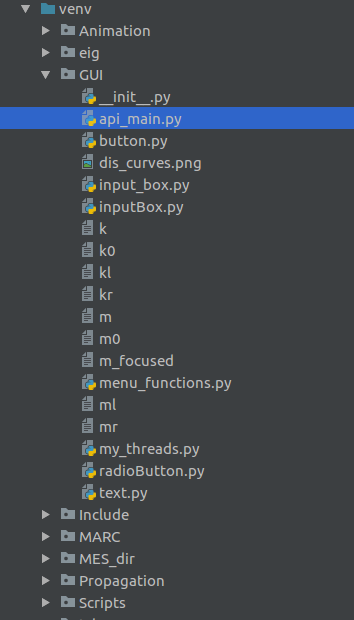
\includegraphics[width=8cm]{Zdjecia/5/kasia/gui_drzewo}
\caption{Położenie $api\_main.py$ w drzewie projektu}
\label{fig:gui_tu_jest}
\end{figure}

Po uruchomieniu programu $api\_main.py$ wyświetlany zostaje graficzny interfejs. Rysunek \ref{fig:gui1} przedstawia wygląd interfejsu zaraz po uruchomieniu.

\begin{figure}[h]
\centering
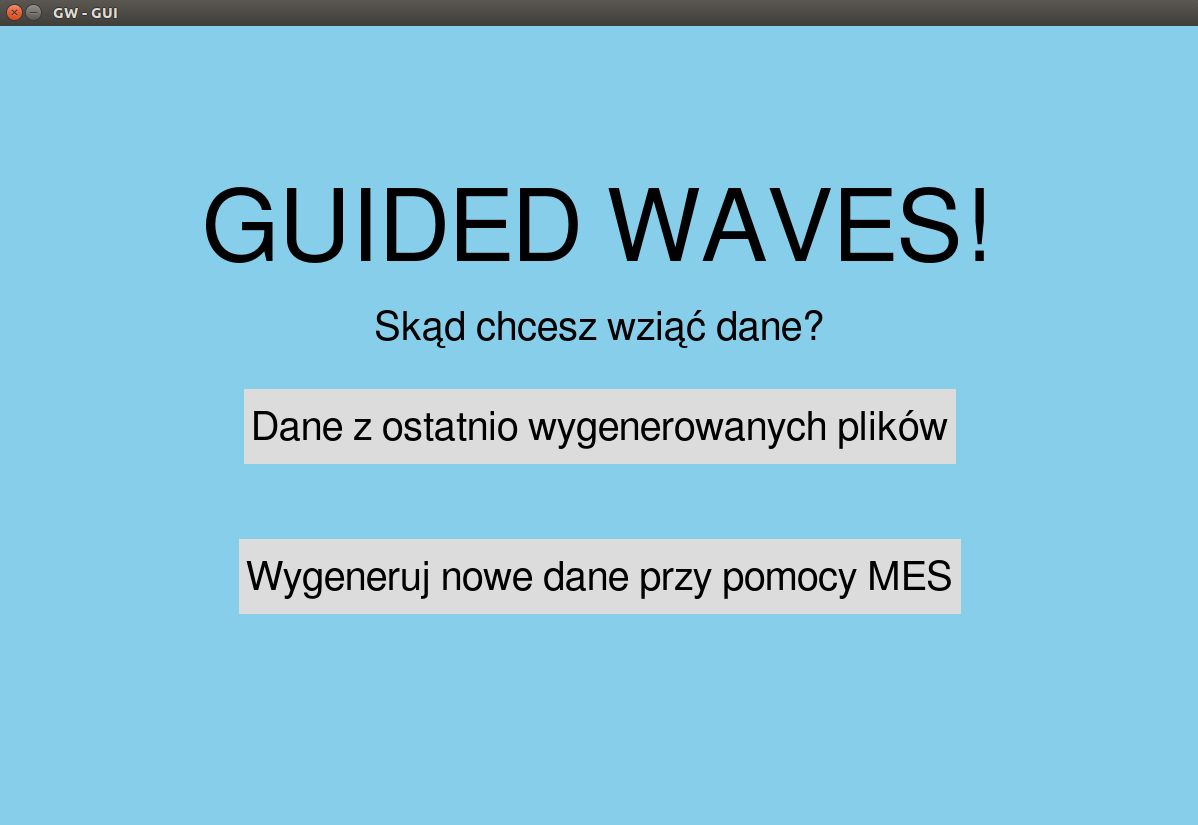
\includegraphics[width=13cm]{Zdjecia/5/kasia/gui1}
\caption{Wybór źródła danych do symulacji}
\label{fig:gui1}
\end{figure}

Po pierwsze użytkownik proszony jest o wybranie, czy chce korzystać z ostatnio wygenerowanych danych czy chce wygenerować nowe dane do symulacji. Nowe dane można również wygenerować później w dowolnym momencie. Po wybraniu opcji "Dane z ostatnio wygenerowanych plików" wyświetlany zostaje komunikat informujący o ładowaniu danych do praogramu (Rysunek \ref{fig:gui2})

\begin{figure}[h]
\centering
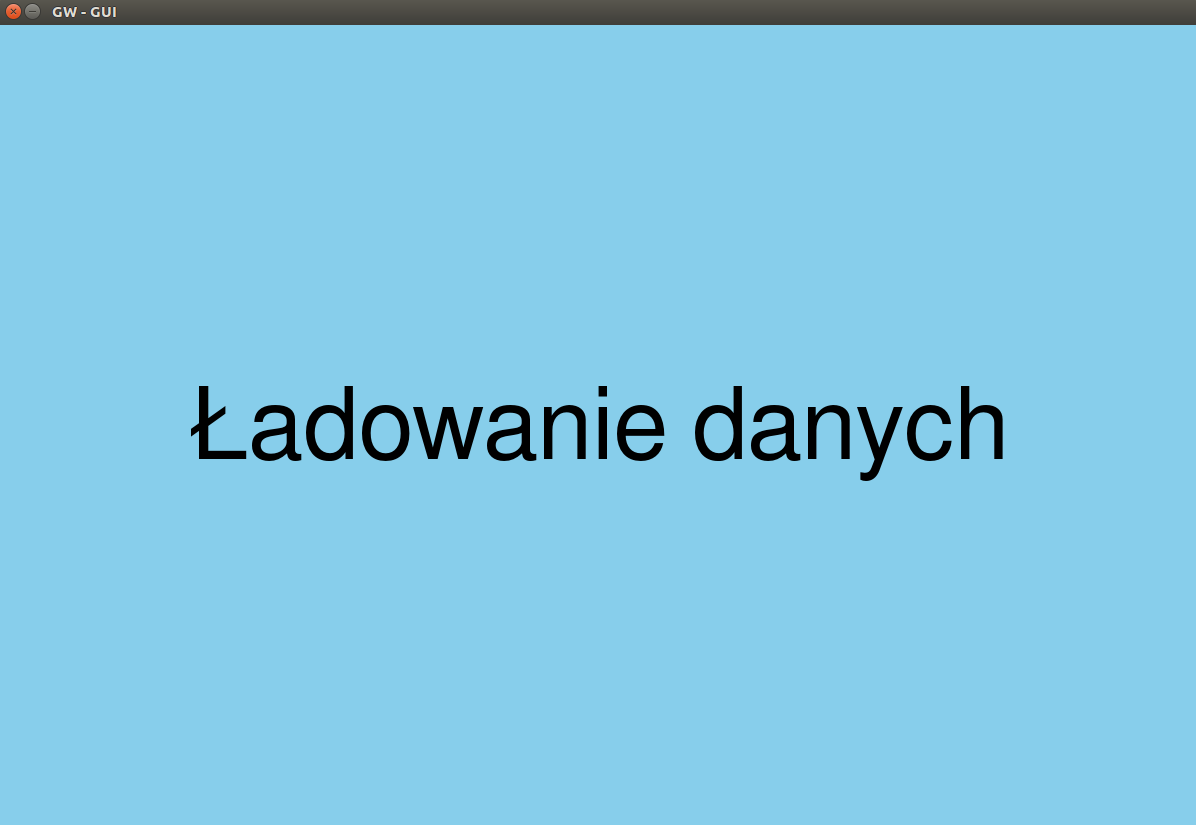
\includegraphics[width=13cm]{Zdjecia/5/kasia/gui2}
\caption{Ekran ładowania danych}
\label{fig:gui2}
\end{figure}

W tym momencie, wygenerowane przez solver dane są wczytywane do programu. A krzywe dyspersji agregowane do odpowiednich obiektów tak jak zostało to opisane w poprzednim podrzdziale. Kiedy ładowanie zostanie zakończone wyswietlany zostaje napis "Krzywe dyspersji" oraz wyświetlane są wczytane krzywe. Przedstawia to rysunek \ref{fig:gui3} \ref{fig:gui4} 

\begin{figure}[h]
\centering
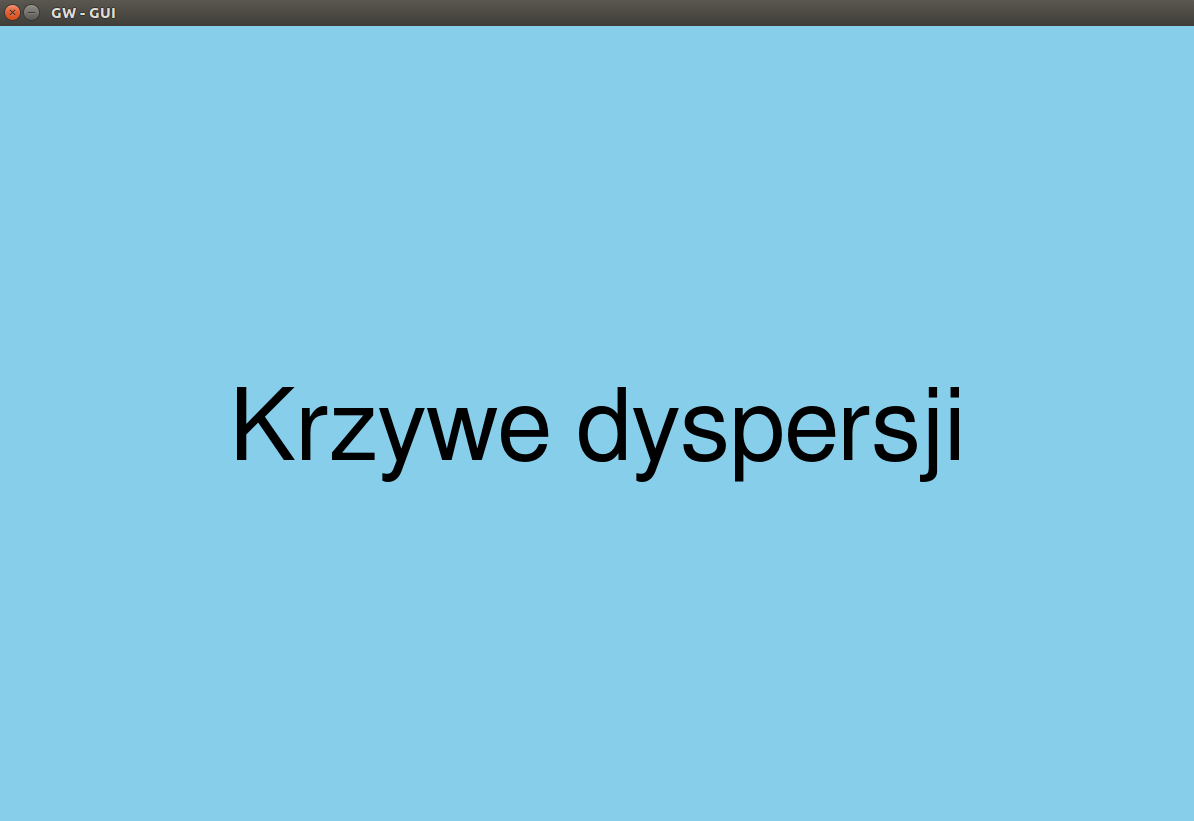
\includegraphics[width=13cm]{Zdjecia/5/kasia/gui3}
\caption{Krzywe dyspersji}
\label{fig:gui3}
\end{figure}

\begin{figure}[h]
\centering
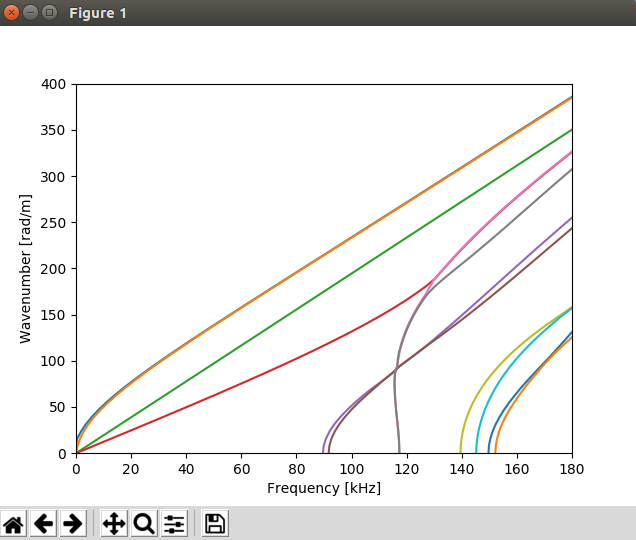
\includegraphics[width=13cm]{Zdjecia/5/kasia/gui4}
\caption{Krzywe dyspersji}
\label{fig:gui4}
\end{figure}

Aby przejść dalej należy zamknać okienko przedstawiające krzywe dyspersji. Następnie wyświetlane jest główne menu interfejsu. Przedstawia je rysunek \ref{fig:gui6}

\begin{figure}[h]
\centering
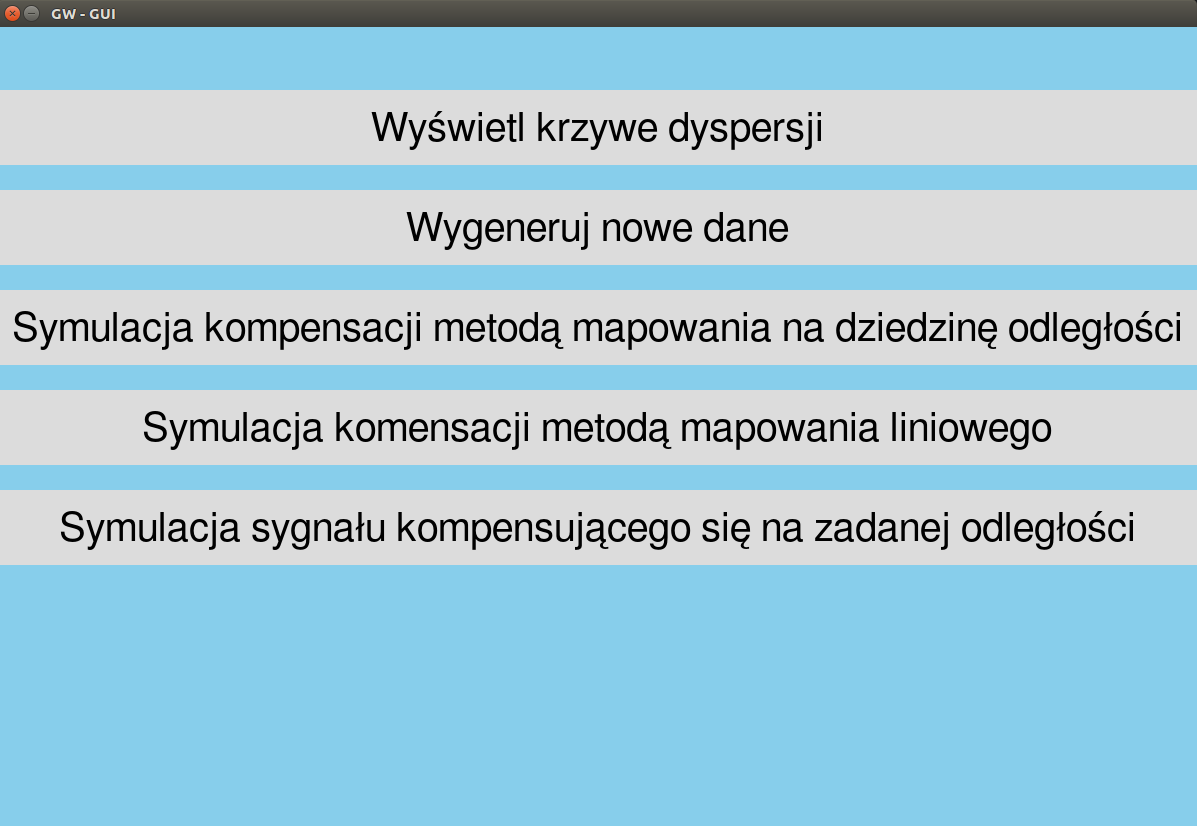
\includegraphics[width=13cm]{Zdjecia/5/kasia/gui6}
\caption{Główne menu programu}
\label{fig:gui6}
\end{figure}

W tej części do wyboru jest pięć opcji. Pierwsza z nich wyświetla okno z krzywymi dyspersji z rysunku \ref{fig:gui4}. Opcja "Wygeneruj nowe dane" przenosi użytkownika do okna z rysunku \ref{fig:gui7}. Okno to zostanie również wyświetlone po wybraniu z okna przedstawionego na rysunku \ref{fig:gui1} opcji "Wygeneruj nowe dane"

\begin{figure}[h]
\centering
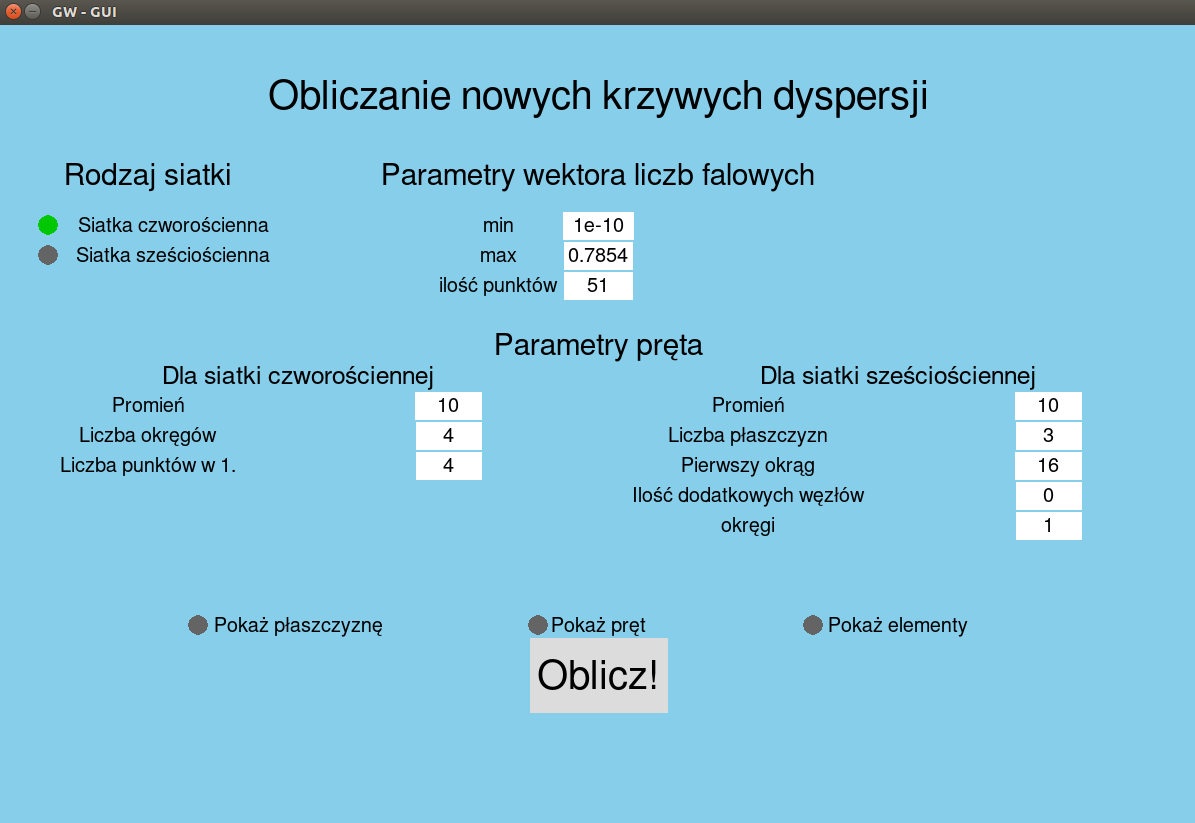
\includegraphics[width=13cm]{Zdjecia/5/kasia/gui7}
\caption{Ekran ustawień siatki}
\label{fig:gui7}
\end{figure}

W tym miejscu można wybrać rodzaj siatki, jaką użytkownik chce wygenerować. Ustawić wszystkie parametry oraz zaznczayć czy chce się wyświetlać benerowaną siatkę zarówno na płaszczyźnie, jak i w postaci pręta czy też elementów skończonych. Po wybraniu interesujących parametrów oraz zatwierdzeniu wyboru poprzez naciśnięcie przycisku "Oblicz" Pojawia się ekran informujący, że obliczenia trwają. Przedstawia to rysunek \ref{fig:gui8}
Ważną kwestią podczas wpisywania parametrów jest podawanie liczb tylko przy pomocy klawiszy znajdujących się nad klawiaturą. Klawiatura numeryczna nie jest obsługiwana, a jej użycie może spowodować błąd oraz zakończenie działania programu. Znacznik szary oznacza, iż dana opcja jest nieaktywna, natomiast znacznik zielony oznacza akywną opcję.

\begin{figure}[h]
\centering
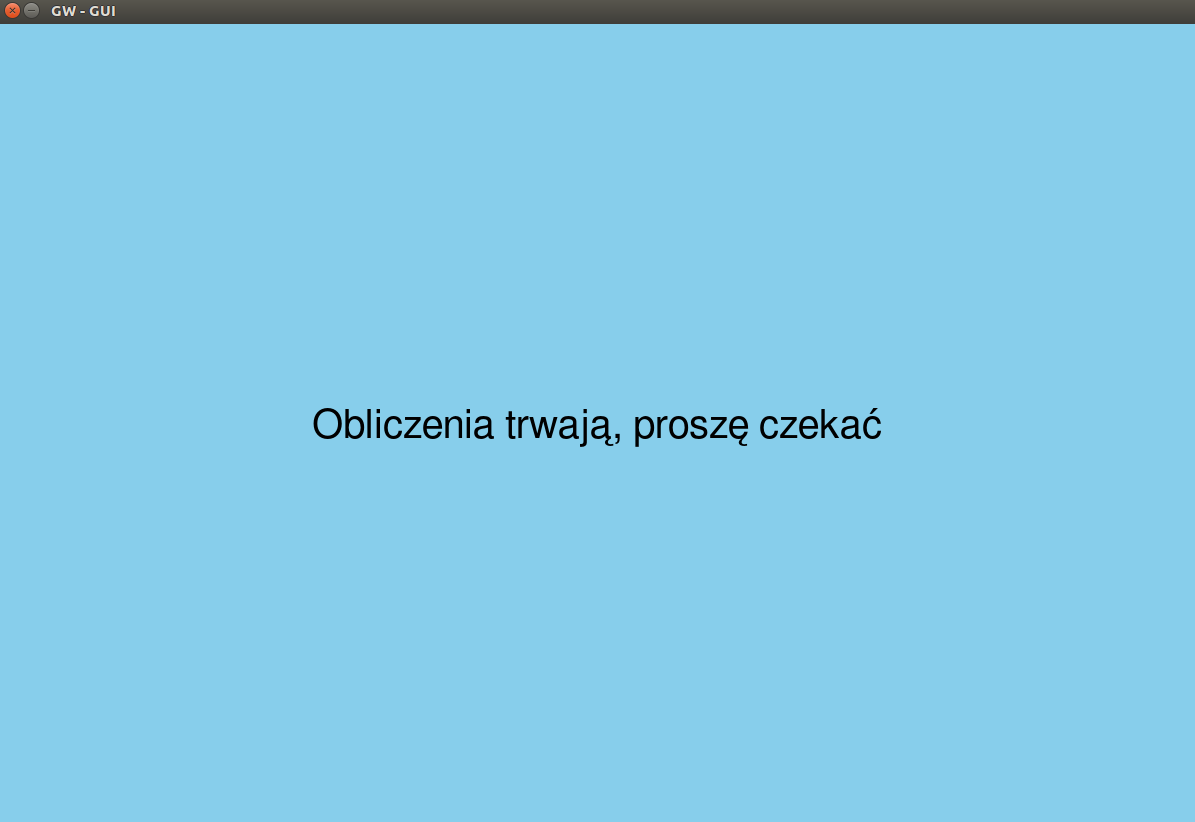
\includegraphics[width=13cm]{Zdjecia/5/kasia/gui8}
\caption{okno programu informujące o trwających obliczeniach}
\label{fig:gui8}
\end{figure}

Gdy siatka zostanie już wygenerowana program wraca do głównego menu z rysunku \ref{fig:gui6}. Kolejne trzy dostępne opcje odpowiadają opisanym już metodom kompensacji dyspersji. W całym interfejsie sygnałem propagującym orz będącym kompensowanym jest sygnał linear chirp pomnożonym przez okno Hanninga z rysunku 4.8. Po wybraniu opcji "Symulacja kompensacji metodą mapowania na dziedzinę odległości pojawia się okno z rysunku \ref{fig:guiKomp1}

\begin{figure}[h]
\centering
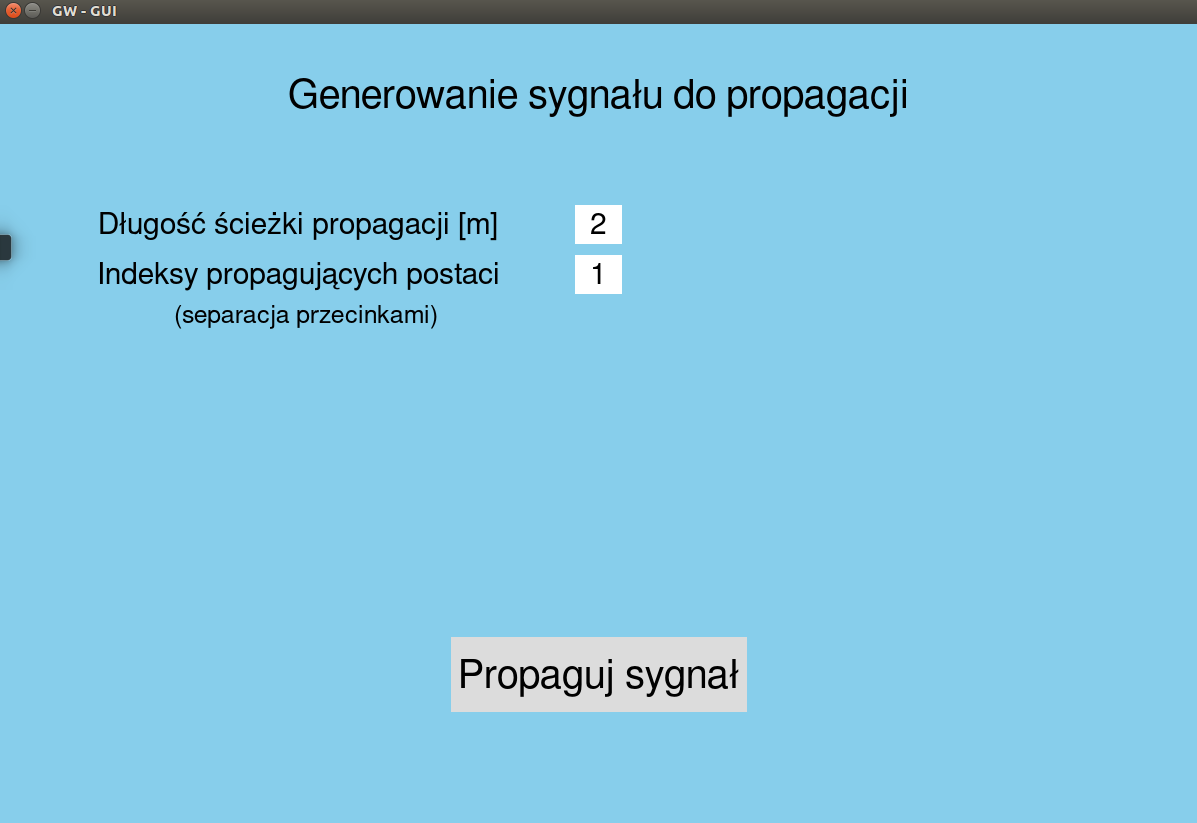
\includegraphics[width=13cm]{Zdjecia/5/kasia/guiKomp1}
\caption{okno programu informujące o trwających obliczeniach}
\label{fig:guiKomp1}
\end{figure}

W tym momencie użytkownik wybiera sygnał, jaki chce wygenerować do symulacji. Zostanie on następnie skompensowany wybraną metodą. Gdy wygenerowany sygnał zostanie skompensowany jest on wyświetlany. Po zamknięciu okienka z wyświetlonymi wynikami, program wraca do głównego menu. Po wybraniu opcji "Symulacja kompensacji metodą mapowania liniowego" program realizuje algorytm analogiczny do właśnie opisanego. Jedyna różnica to metoda jaką kompensowany jest sygnał. Wybranie opcji "Symulacja sygnału kompensującego się na zadanej odległości" otwiera okno przedstawione na rysunku \ref{fig:guiLast}

\begin{figure}[h]
\centering
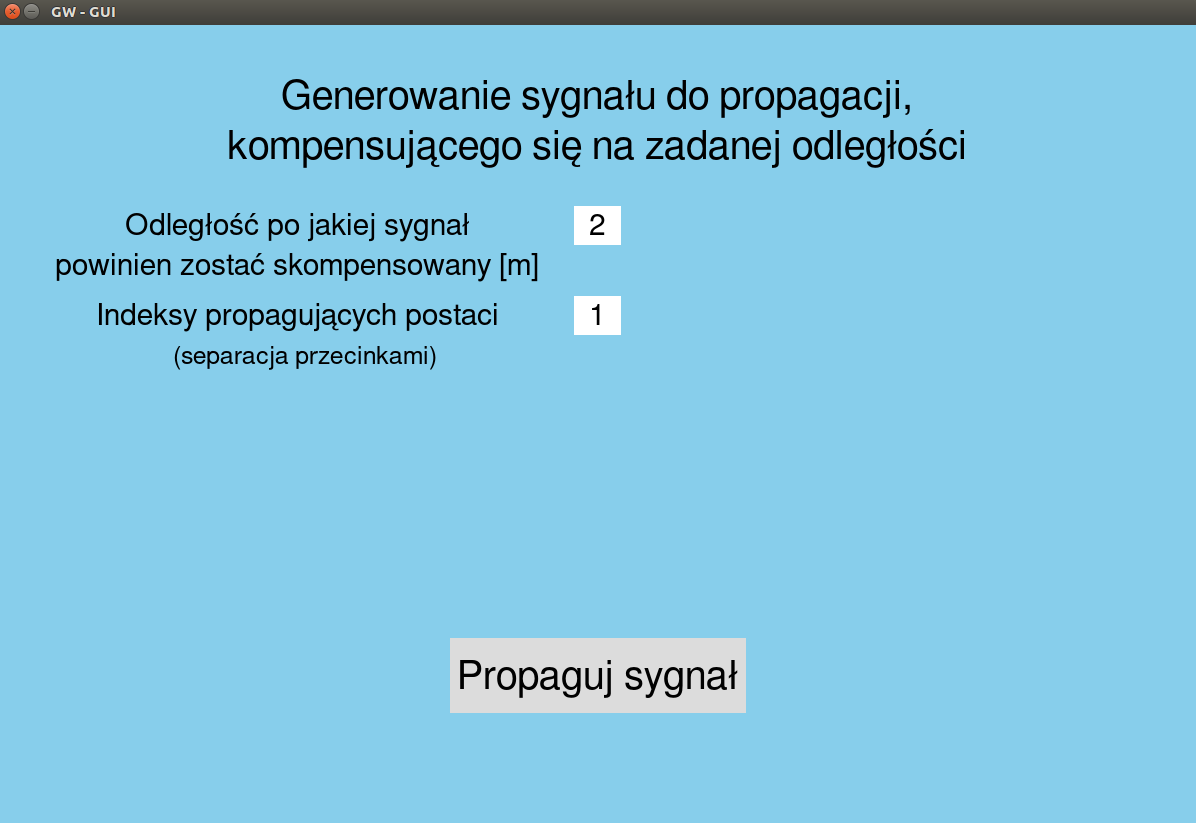
\includegraphics[width=13cm]{Zdjecia/5/kasia/guiLast}
\caption{okno programu informujące o trwających obliczeniach}
\label{fig:guiLast}
\end{figure}

Po wpisaniu odpowiednich parametrów oraz wykonaniu stosownych obliczeń wyświetlany jest wygenerowany sygnał. Po zamknięciu okna wyświetlającego wyniki pojawia się  okno pozwalające na ustawienie danych propagacji, tak aby można było zaobserwować zachowanie wygenerowanego sygnału po propagacji (rys. \ref{fig:guiLast2})

\begin{figure}[h]
\centering
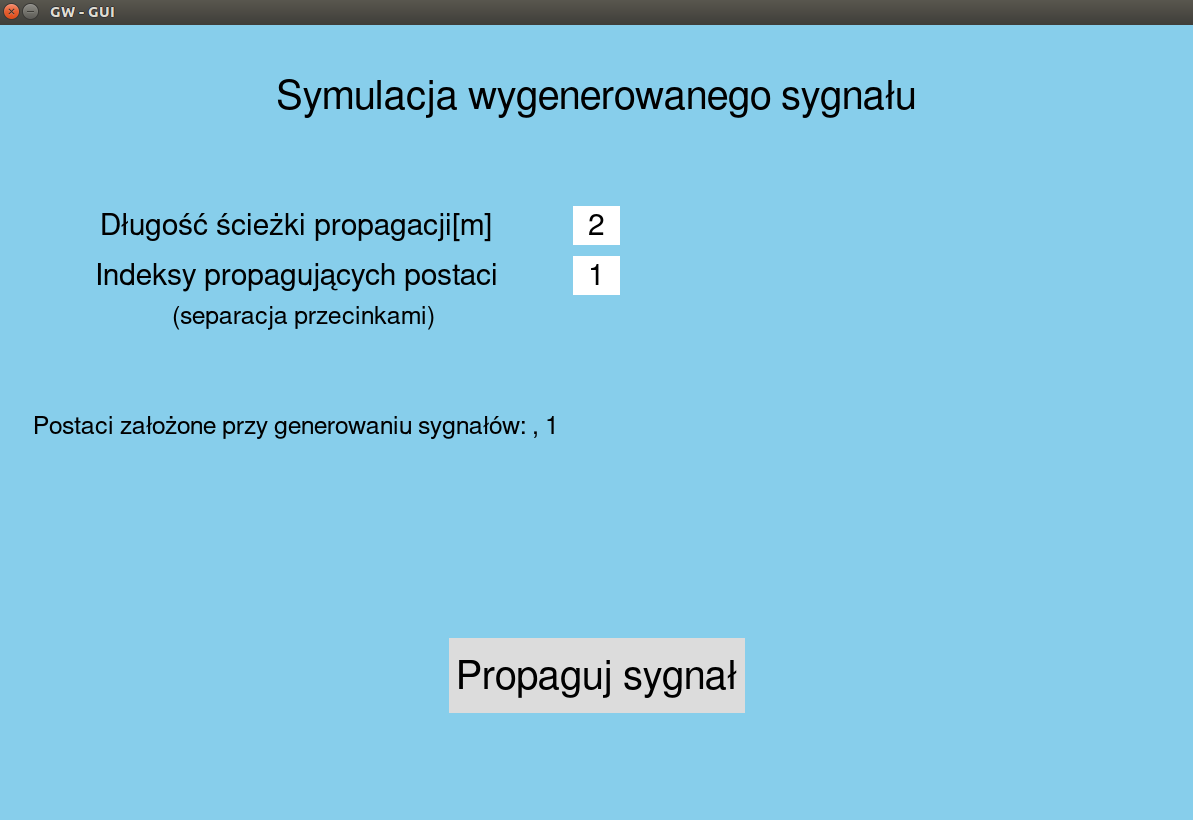
\includegraphics[width=13cm]{Zdjecia/5/kasia/guiLast2}
\caption{okno programu informujące o trwających obliczeniach}
\label{fig:guiLast2}
\end{figure}

Po skończonych obliczeniach wyświetlany jest otrzymany sygnał.